\section{Introduction}

    à partir d'un jeu de donnée fourni par the World Bank Group en 2007, nous avons essayé de déterminer certaines corrélations et de faire apparaitre des liens parmis ces données.
    Ces dernières contiennent des informations concernant 48 atributs sur 209 pays.
    Cependant certaines données sont manquantes, la première étape a donc été de trier les données pour ne récupérer que des données valides.
    Il aurait pu être intéressant d'essayer de retrouver certaines données manquantes, mais nous n'avons pas choisi d'effectuer cette étude.
	Durant notre étude, nous n'avons travaillé que sur le fichier countries\_2007\_all.csv. Nous avons préféré supprimer uniquement les données manquante à notre étude plutôt que de trier un jeu de données déjà réduit.
	    
\section{Tri des données}
    Nous savions que, quelque soit l'étude choisie, il faudrais éliminer un certains nombre d'attributs et un certains nombre de pays pour lesquelles les données manquent.
    Pour effectuer cette opération, nous avons mis en place une chaîne de selection permettant de trier précisément, par selection, les attributs puis les pays à inclure dans l'étude. Une solution alternative aurait été de trier uniquement les attributs interessant, puis supprimer tous les pays pour lesquelles des données manquent, mais afin de pouvoir vérifier quels pays doivent être enlevés, la première solution à été préférée.
    Un accent à été mis sur la visualisation des données manquantes. Grâce à des selecteurs, nous avons mis en place une chaîne permettant de connaître précisement le nombre de pays pour lesquelles manque un attribut, et le nombre d'attributs qui manquent à un pays.
    Grâce à ces selecteurs, nous faisions les tris necessaires afin d'obtenir uniquement un ensemble de données sans données manquantes.\\
	La figurre suivante correspond au diagramme nous permettant de trier les jeux de données afin de sélectionner les colonnes à étudier et de supprimer éléments contenant des valeurs manquantes dans les colonnes étudiées.\\	
	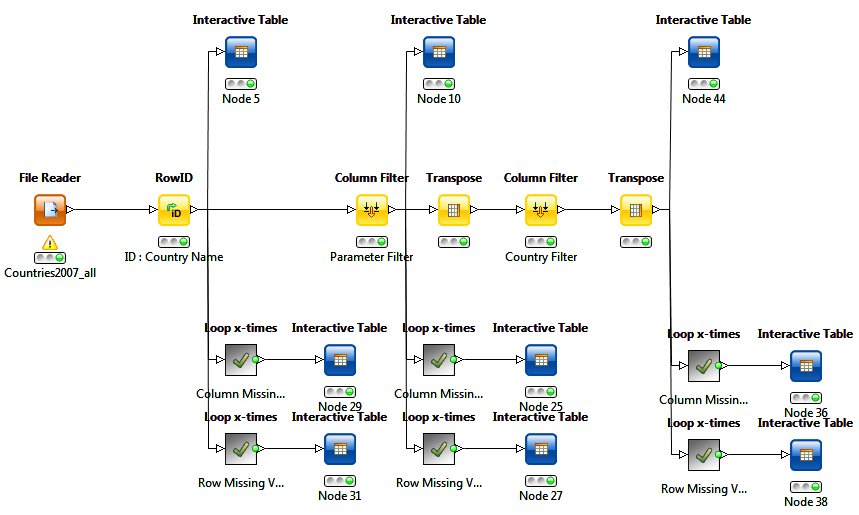
\includegraphics[width=0.9\textwidth]{Tri.png}	\\
	Dans ce diagramme, nous commençons par lire le jeu de données complet à l'aide d'un \textbf{File Reader}. Le bloc \textbf{RowID} nous permet ensuite de définir la colonne des noms de pays comme indexe du jeu de données. Nous avons ensuite utilisé à deux reprises le composant \textbf{Loop x-times} comme simple conteneur de blocs : afin de simplifier le diagramme général, nous avons encapsulé dans ce bloc les éléments suivants :\\
	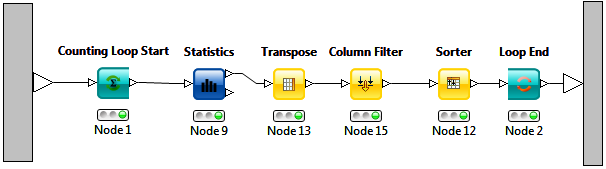
\includegraphics[width=0.9\textwidth]{Loop.png}\\
	Nous n'utilisons ici le composant \textbf{Loop x-times} que par soucis de lisibilité du diagramme général, nous avons fixé le nombre d'itérations à 1.
	Cette fonction permet de compter le nombre de valeurs manquantes par colonne. Par exemple, on peut voir ci-dessous le nombre de valeurs manquantes par colonne dans le jeu de donnée de base : \\
	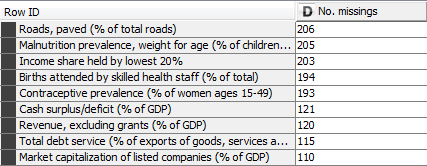
\includegraphics[width=0.9\textwidth]{ColumnMissing.png}\\
	Nous utilisont alors un élément \textbf{column Filter} afin de supprimer les colonnes inutiles à notre étude.\\
	Le même principe est appliqué à pour la suppression des pays dont les valeurs dans les colonnes étudiées sont manquantes. Nous commençons par tranposer la table pour avoir les pays en colonnes et nous filtrons alors les colonnes contenant des valeurs manquantes.
		
		
\section{Visualisation, corrélation, choix des dimensions, }

    Nous avons fais plusieurs comparaison, afin d'essayer d'établir des corrélation avec le pourcentage d'utilisation d'internet.
    \begin{itemize}
        \item La première comparaison à été faite avec le GDP et le GNI.
        \item La seconde comparaison à été faite avec le pourcentage de souscription à un forfait mobile.
        \item La troisiéme comparaison à été faite avec le temps requis pour démarrer une entreprise.
    \end{itemize}

    \subsection{Normalisation}
        Afin d'avoir des distances significatives, pour établir des cluster cohérent, les données sont normalisé.
        Si la normalisation n'est pas faite un des attributs à un domaine bien plus grand que l'autre, ce qui en résulte sur des clusters qui semblent ne pas dépendre de l'attributs qui à le domaine le plus grand.
        En effet la distance etant bien plus grand sur une dimension que sur l'autre, le nuage de point peut être imaginé comme une longue bandelette, et Knime découpe les cluster selon une seule dimension.
        La normalisation permet donc, sans modifier la répartition des points, d'avoir des calculs de distance plus efficaces, et donc des clusters cohérents.
        
    \subsection{Echelle logarithmique}
        Dans le cas du GDP et du GNI, les données sont réparties de telles façon qu'un grand nombre de pays se trouve avoir des valeurs trés faibles, tandis que peu ont un GDP ou un GNI trés fort.
        La répartition selon cette dimension semblait logarithmique, nous avons donc essayé d'utiliser une echelle logarithmique afin d'améliorer la visualisation des données.
        Grâce à cette nouvelle répartition, le nuage de point était réparti de manière bien plus homogéne.
        
    \subsection{Internet Utilisation - GDP\/GNI}
        La comparaison entre GDP et GNI n'as pas permis de déceler de correlation évidente, à part des conclusions déjà connues concernant les extremes : un pays avec un trés faible GDP n'auras pas une forte utilisation d'internet, de même, un pays avec un fort GDP auras forcément une certaine utilisation d'internet.
        En revanche, on peut établir des groupes de pays ayant des caractéristiques communes :\\
        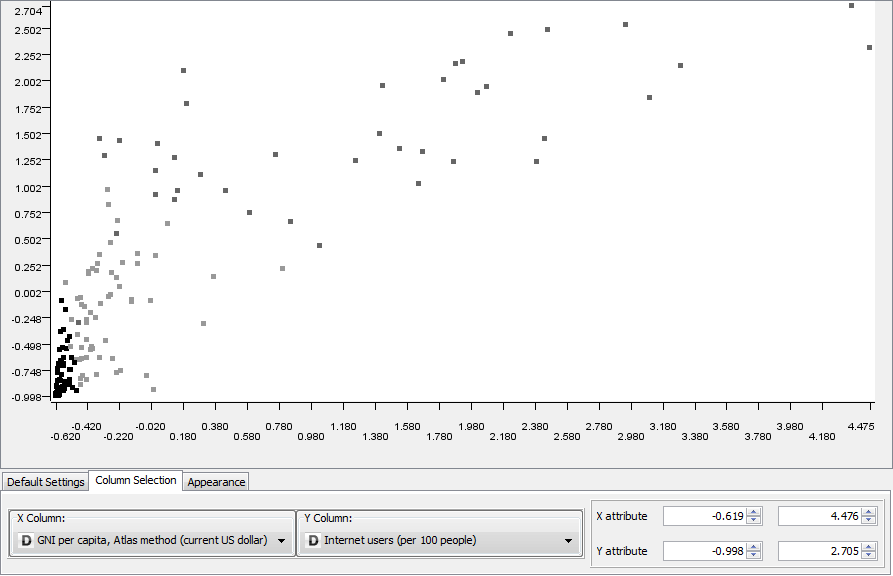
\includegraphics[width=0.9\textwidth]{InternetGNI.png}\\
		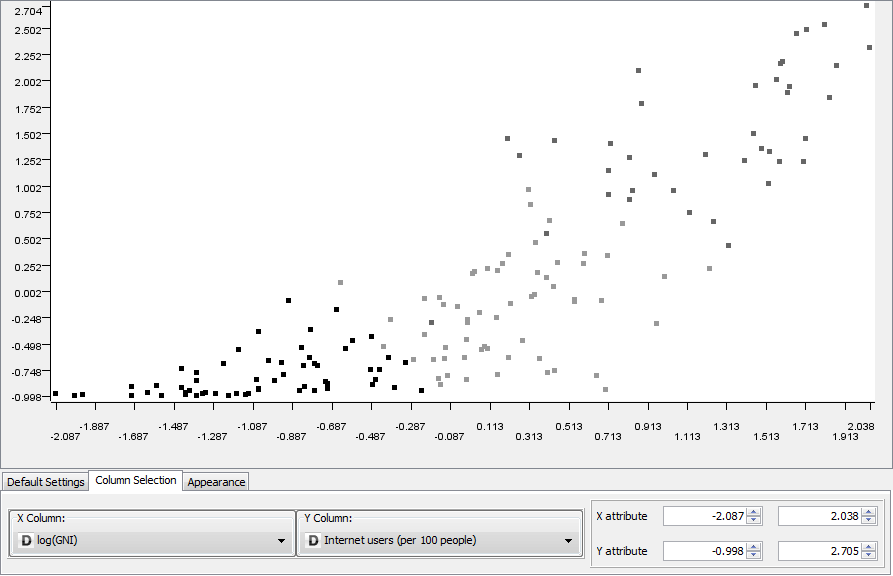
\includegraphics[width=0.9\textwidth]{InternetLogGNI.png}\\
        
		Les résultats avec le GDP étant similaires mais moins visibles, nous ne présentons ici que ceux du GNI.
		La vue suivante représente la vue du \textbf{Hierarchical Clustering}. Cette vue nous a permis de définir le nombre de clusters à créer. Nous nous sommes limités à 3 clusters, bien que cette valeur soit située avant le point d'inflexion de la courbe de distance car la distance entre 3 et 4 clusters était déjà trop faible et ne justifiait pas la création d'un nouveau groupe de données.\\
		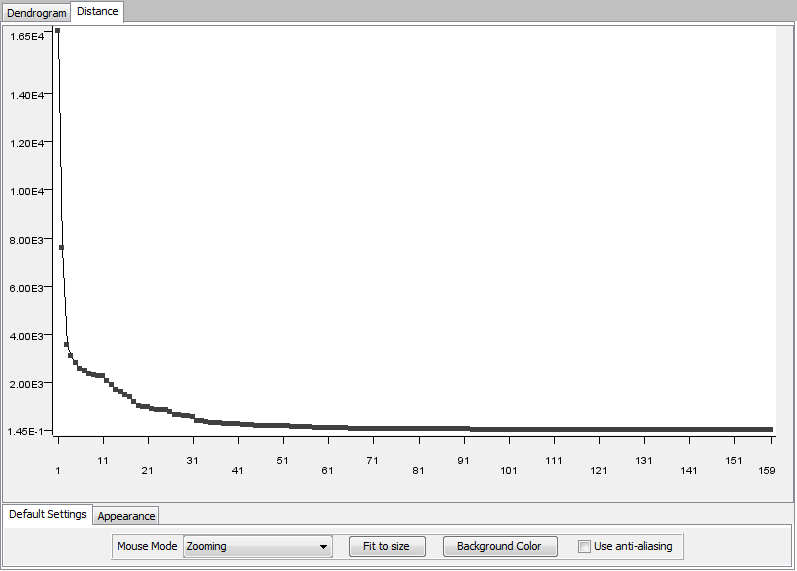
\includegraphics[width=0.9\textwidth]{distanceGNI.png}\\

    \subsection{Internet UTilisation - Mobile subscription}
        Cette c


\section{Cluster non guidé}

\section{Cluster guidé et prédiction appartenance}
